\chapter{Trabalhos Relacionados}\label{cap:trabalhos}

A floresta amazônica é tema recorrente em diversas áreas de pesquisa, incluindo a área de sensoriamento remoto. Trabalhos vindos desta área costumam utilizar técnicas computacionais que pertencem ao estado da arte para analisar imagens que cobrem grandes áreas, sejam essas de espectro visível ou mesmo de RADAR ou LIDAR, e inferir as mais diversas informações sobre as regiões estudadas.

Trabalhos como os de \citeonline{almeidafilho:1998}, \citeonline{vasconcelos:2001}, \citeonline{lu:2012} e \citeonline{ferreira:2012} se utilizam de imagens com 6 bandas multiespectrais e 1 banda termal do satélite LANDSAT da região amazônica para determinar a cobertura de terreno das áreas inspecionadas. Estes trabalhos têm foco nos tipos de vegetação que cobrem o terreno, classes tais como floresta, capoeira, vegetação secundária, ou até mesmo espécies e grupos de plantas. Há trabalhos mais elaborados, como o de \citeonline{espiritosanto:2005}, que se utiliza das mesmas imagens do satélite LANDSAT, mas analisa amostras multitemporais, ou seja, imagens da mesma região em diversos sobrevoos do satélite, com o objetivo conseguir informações sobre mudanças na cobertura vegetal do terreno.

Há ainda trabalhos como o de \cite{azevedo:2014}, que utiliza como fonte de dados o satélite COSMO-SkyMed,  que disponibiliza imagens duais multitemporais da região amazônica. Estudos como o de \citeonline{latorre:2007} vão além e mesclam os dados de diversas fontes diferentes, utilizando técnicas de fusão de imagens.

Apesar dos resultados alcançados, os trabalhos sobre a classificação de imagens da floresta amazônica geralmente avaliam a cobertura vegetal da região, sem qualquer menção a elementos antrópicos, utilizando para isso imagens termais ou multiespectrais de diversos satélites. Dada a natureza relativamente lenta das mudanças de cobertura vegetal de terreno e o tamanho das áreas estudadas, é compreensível que satélites sejam utilizados.

Para o trabalho aqui apresentado, no entanto, os objetos de interesse mudam rapidamente, e a grande cobertura de área proporcionada por imagens de satélite deve dar lugar a imagens feitas por veículos aéreos, com maior proximidade e disponibilizadas com mais rapidez em uma missão real de patrulhamento ambiental. A base de imagens disponível para o trabalho é composta exclusivamente por imagens de espectro visível, por isso, muitas das técnicas e conclusões dos trabalhos citados acima não são prontamente transferíveis para este trabalho.

Os trabalhos relacionados apresentados nesta seção foram divididos primeiramente por assunto: de início, nos concentramos nos trabalhos publicados em segmentação de imagens que são considerados estado da arte, uma vez que esta é o primeiro desafio técnico a ser enfrentado pelo trabalho proposto. Depois, fazemos o levantamento de trabalhos relevantes sobre classificação de imagens aéreas. Em uma etapa posterior, investigamos trabalhos relacionados na área de detecção de anomalias.

As seções a seguir apresentam os trabalhos relacionados em ordem própria.  A seção \ref{sec:trSegmentacao} apresenta os trabalhos sobre segmentação de imagens de acordo com a ordem apresentada no trabalho de comparação realizado por \citeonline{arbelaez:2011}, explanado com mais detalhes em seguida. As seções \ref{sec:trClassificacao} e \ref{sec:trAnomalias} apresenta os trabalhos relacionados sobre classificação de imagens aéreas e detecção de anomalias, ambas em ordem cronológica de publicação.

Cada artigo é descrito com suas características, vantagens e desvantagens. No fim de cada seção, é apresentada uma tabela de comparação entre os trabalhos levantados.

\section{Segmentação de imagens}\label{sec:trSegmentacao}

Os trabalhos relacionados nesta seção foram escolhidos por terem obtido os maiores índices de precisão e revocação em uma base de dados de imagens naturais bastante conhecida pela comunidade de processamento de imagens, \textit{Berkeley Segmentation Data Set and Benchmarks 500}, também conhecida como BSDS500. Uma comparação entre os mais promissores algoritmos de segmentação de imagens foi realizada por \citeonline{arbelaez:2011}, consistindo na segmentação das imagens presentes no BSDS500 manualmente por seres humanos, e depois segmentadas pelos diversos algoritmos testados. A precisão e revocação de cada algoritmo são obtidas através de comparação com a segmentação manual.

Para reduzir ainda mais o número de algoritmos a serem inspecionados para este trabalho, a revisão de \citeonline{yuan2:2013} compara os mesmos algoritmos que \citeonline{arbelaez:2011} investigaram, mas dessa vez em uma base de imagens aéreas. A metodologia é a mesma usada no BSDS500, mas com uma base especializada. Os algoritmos com os melhores resultados foram selecionados para serem utilizados na construção deste trabalho de pesquisa, e coincidem com os resultados do trabalho de \citeonline{arbelaez:2011}. Os seis algoritmos selecionados serão discutidos a seguir.

%%%% JSEG %%%%

O trabalho de \citeonline{deng:2001} trata de um algoritmo chamado JSEG (acrônimo para \textit{J Segmentation}), que obtém a segmentação da imagem em duas etapas. A primeira é a quantização das cores da imagem em um número bem menor que o número original, cerca de 16 milhões, em uma imagem de 24 bits, para um número entre 10 e 20 cores na imagem resultante. Esta etapa é responsável por criar uma espécie de mapa de classes, baseada nas cores quantizadas e ignorando a distribuição espacial destas mesmas cores (figura \ref{fig:jseg_classmap}).

\begin{figure}[h]
  \centering
  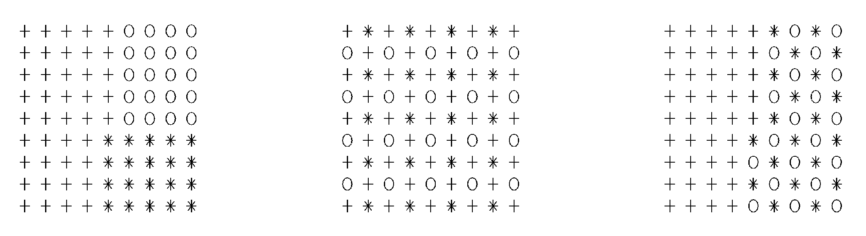
\includegraphics[scale=1]{imgs/jseg_classmap}
  \caption[Exemplos de mapas de classes do algoritmo JSEG]{Exemplos de mapas de classes do algoritmo JSEG, criado a partir da quantização de cores. Fonte: \cite{deng:2001}}
  \label{fig:jseg_classmap}
\end{figure}

A segunda etapa consiste na segmentação espacial do mapa de classes sem considerar a similaridade cromática dos pixels. Para que isto seja possível, primeiramente é encontrado o valor para uma variável $J$. Seja $Z$ o conjunto de todos os $N$ pontos do mapa de classes, temos que $z = (x,y), z \in Z$ e $m$ seja a média, dada por

\begin{equation}
	\displaystyle m = \frac{1}{N} \sum_{z \in Z} z
\end{equation}

Supondo que $Z$ é dividido entre $C$ classes, $Z_i$, $i = 1,...,C$. A média $m_i$ dos $N_i$ pontos da classe $Z_i$ pode ser definida por

\begin{equation}
	\displaystyle m_i = \frac{1}{N_i} \sum_{z \in Z_i} z
\end{equation}

Podemos definir $S_T$ como:

\begin{equation}
	\displaystyle S_T = \sum_{z \in Z} || z - m ||^2
\end{equation}

e $S_W$, a variância total de pontos pertencentes à mesma classe, como:

\begin{equation}
	\displaystyle S_W = \sum_{i=1}^C \sum_{z \in Z} || z - m ||^2
\end{equation}

Podemos, então, calcular $J$ por

\begin{equation}
	\displaystyle J = \frac{S_T - S_W}{S_W}
\end{equation}

Com isso, temos valores de $J$ maiores para imagens com regiões de cores mais homogêneas. Quando a distribuição de classes é mais homogeneamente distribuída pela imagem, $J$ assume um valor baixo. POsteriormente, um método de crescimento de região para segmentar a imagem com base no valor \textit{J} é aplicado, determinando as regiões finais da imagem.

O algoritmo ainda permite que o utilizador especifique o tamanho da janela para computar o valor de \textit{J}, o que torna o método bastante flexível para imagens de naturezas diferentes. Em imagens aéreas de escala considerável, como as utilizadas neste trabalho, pode-se usar uma janela diminuta, já que os detalhes importantes podem ser bem pequenos. Para diminuir super-segmentação, os segmentos encontrados na segunda etapa são fundidos de acordo com seus histogramas coloridos.

%%%% Meanshift %%%%

A abordagem utilizando mean-shift (ou mudança de média, numa tradução literal) desenvolvida por \citeonline{comaniciu:2002} oferece uma ferramenta interessante para resolver o problema de segmentação de imagens. Em um primeiro momento, uma filtragem por mean-shift para suavização da imagem é aplicada e os dados desta imagem pós-filtrada são projetados em um domínio $d$-dimensional que considera informações espaciais e cromáticas. Estas informações são agrupadas utilizando um critério de proximidade. Nesta etapa, as amostras cuja distância no domínio espacial estão abaixo de $h_s$, e no domínio de cores estão abaixo de $h_r$, serão agrupados em um mesmo \textit{cluster}.

Após a convergência do processo de agrupamento, os \textit{clusters} menores que um tamanho mínimo estipulado são absorvidos pelo \textit{cluster} adjacente com maior similaridade, seguindos os mesmos critérios do processo de agrupamento original. Por fim, os segmentos são delimitados utilizando as bordas dos \textit{clusters} encontrados. Parâmetros como distancia espacial, distancia de cores e o tamanho mínimo dos \textit{clusters} podem ser determinados pelo usuario, para adequar o algoritmo ao problema em questão. A figura \ref{fig:meanshift_exemplo} exemplifica o processo de segmentação utilizando o algoritmo de mean-shift para uma imagem hipotética em tons de cinza.

\begin{figure}[h]
  \centering
  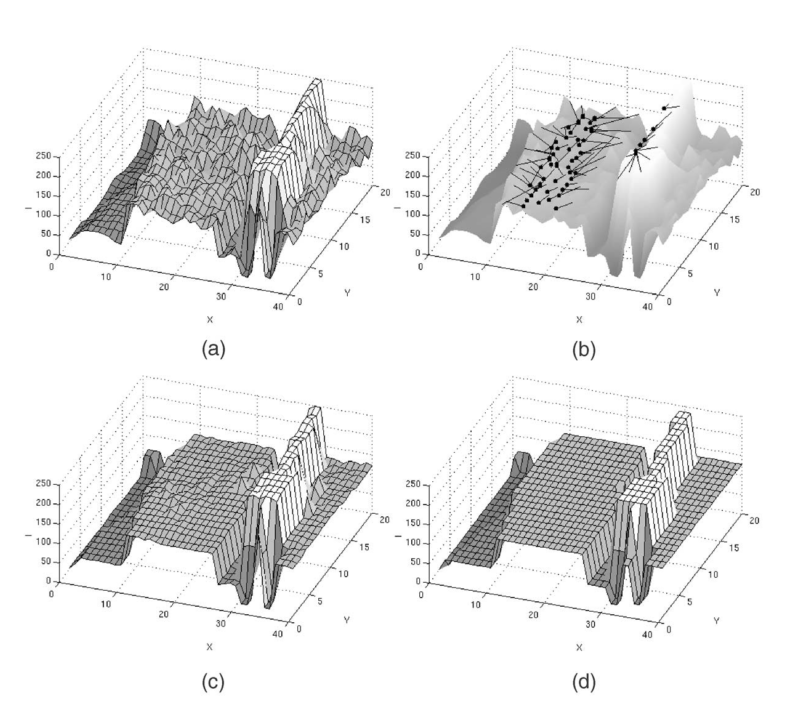
\includegraphics[scale=0.5]{imgs/meanshift_exemplo}
  \caption[Exemplo de segmentação mean-shift em uma imagem em tons de cinza]{Exemplo de segmentação mean-shift em uma imagem em tons de cinza. (a) Imagem de entrada. (b) Filtragem mean-shift para suavização. (c) Resultado do agrupamento sob parâmetros $h_s$ e $h_r$. (d) Resultado da segmentação. Fonte: \cite{comaniciu:2002}}
  \label{fig:meanshift_exemplo}
\end{figure}

%%%% MSEG %%%%

O algoritmo \textit{Multi-resolution Region Merging Segmentation} (MSEG), descrito por \citeonline{felzenszwalb:2004}, é amplamente usado pela comunidade de sensoriamento remoto. Baseado em grafos, este algoritmo tem preocupação com a previsibilidade da segmentação e com o seu custo computacional, da ordem de O(n log n).

O MSEG representa o problema de segmentação como um grafo $G = (V,E)$ não direcionado, onde cada vértice $v \in V$ corresponde a um pixel da imagem a ser segmentada, e cada aresta $(v_i, v_j) \in E$ conecta dois vértices $v_i$ e $v_j$. As arestas possuem um peso $w(v_i, v_j)$, um valor não-negativo que representa a diferença entre os vértices $v_i$ e $v_j$. Nesta abordagem, uma segmentação $S$ é a partição de $V$ em regiões de tal forma que cada região $C \in S$ corresponde a um componente conectado no grafo $G' = (V, E')$, onde $E' \subseteq E$. O conceito principal gira em torno dos pesos entre os vértices de uma mesma região, que devem ser baixos, enquanto os pesos altos devem ser utilizados para encontrar bordas entre as regiões.

O aumento na heterogeneidade no momento da junção de um par de segmentos é computado como uma soma ponderada de medidas de coloração e morfologia. O procedimento de junção é realizado iterativamente, e  junta os pares de segmento que resultam no menor aumento de heterogeneidade possível, até que a soma exceda um limiar, que pode ser parametrizado pelo utilizador. Um parâmetro é utilizado para definir a escala observada na segmentação, o que influi no tamanho e no número dos segmentos resultantes.

A principal vantagem deste método reside no desempenho computacional, com custo próximo ao linear em função do número de pixels da imagem. Os autores do algoritmo sugerem que ele seja perfeitamente adequado para o processamento de imagens de grandes dimensões, ou mesmo segmentação de vídeo em tempo real.

%%%% SRM %%%%

O algoritmo de segementação baseada em crescimento/junção de regiões \textit{Statistical Region Merging} (SRM), publicado por \citeonline{nock:2004}, utiliza um procedimento simples de junção acompanhado por uma operação de ordenação para segmentar imagens com eficiência. A ordenação da junção de regiões é realizada através de um algoritmo guloso, que percorre sempre o menor custo de caminhamento entre pixels de 4-vizinhança (pixels vizinhos ao norte, sul, leste e oeste, ignorando as diagonais). O custo do caminhamento é obtido através de uma função objetiva, definida por

\begin{equation}
	\displaystyle f_a(p, p') = |p_a - p'_a|
\end{equation}

onde $f_a(p, p')$ é a distância máxima entre os canais de cores dos pixels $p$ e $p'$. Esta simples função, segundo o artigo de \citeonline{nock:2004}, não representa um problema, pois evidências experimentais mostram que o ganho ao usar uma função mais objetiva, como o kernels de convolução, não melhoram significativamente os resultados.

Duas regiões da imagem são unidas se os valores médios dos pixels das duas regiões estão mais próximos que um limiar previamente definido. A coesão da segmentação pode ser controlada por um parâmetro $Q$ definido pelo usuário, que também interfere na muito embora.

Segundo os autores, este algoritmo sofre de um problema descrito como sobrejunção (do inglês \textit{overmerging}), ou seja, ele tende a juntar duas regiões que deveriam ser separadas. O algoritmo, em compensação, parece não sofrer de subjunção, quando uma região é desnecessariamente dividida em diversos segmentos.

%%%% FSEG %%%%

O trabalho de \citeonline{yuan:2013} apresenta um algoritmo chamado \textit{Factorisation-based segmentation} (FSEG). O FSEG primeiramente computa o histograma espectral para cada pixel da imagem, que é um amalgama de diversas respostas aos filtros em uma janela local. Esse algoritmo é baseado na proposta de que cada característica pode ser aproximada por uma combinação linear de diversas características representativas e suas combinações ponderadas. Por fim, um pixel é dito pertencente à região com maior peso. O algoritmo FSEG utiliza decomposição de valores singulares e fatoração de matrizes não-negativas para aumentar a eficiência computacional da segmentação, o que é atrativo quando o tempo de processamento é um fator importante.




O algoritmo gPb-owt-ucm (\textit{Oriented Watershed Transform Ultrametric Contour Maps with globalPb}) introduzido por \citeonline{arbelaez:2011} realiza segmentação em várias etapas. Primeiramente a técnica combina informações de intensidade, textura e coloração para computar vetores que servirão como  detectores de contorno. Posteriormente, uma técnica de \textit{watershed} é aplicada à saída do detector de contornos para produzir uma segmentação hierárquica da imagem. Uma vantagem importante desta técnica é a possibilidade de ajustar a escala de segmentação, portanto o usuário pode escolher uma escala que mais se adequa ao tipo de imagem do problema, evitando segmentação excessiva da imagem.

A tabela \ref{tab:sumarioSegmentacao} exibe os resultados encontrados por \citeonline{yuan2:2013}, juntamente com uma descrição das características das diversas técnicas de segmentação de imagens levantadas neste trabalho.

\begin{table}[h]
\ABNTEXfontereduzida
\centering
\begin{tabulary}{\linewidth}{|L|L|R|R|}
\hline
\textbf{Técnica} & \textbf{Características} & \textbf{Prec. bordas} & \textbf{Prec. regiões } \\ \hline
Manual      & Não aplicável    & 69\% & 84\% \\ \hline
gPb-owt-ucm & Cor, borda       & 65\% & 69\% \\ \hline
FSEG        & Textura          & 61\% & 66\% \\ \hline
SRM         & Cor, intensidade & 60\% & 60\% \\ \hline
JSEG        & Cor, borda       & 56\% & 66\% \\ \hline
MSEG        & Cor, morfologia  & 57\% & 50\% \\ \hline
Mean-shift  & Cor, posição     & 58\% & 48\% \\ \hline
\end{tabulary}
\caption{Comparação entre as técnicas de segmentação de imagens, ordenados por desempenho decrescente, conforme resultados em \citeonline{yuan2:2013} }
\label{tab:sumarioSegmentacao}
\end{table}

Tanto na revisão feita por \citeonline{arbelaez:2011} com a base de imagens naturais BSD500, quanto na comparação feita por \citeonline{yuan2:2013} em uma base de imagens aéreas, o algoritmo gPb-owt-ucm de \citeonline{arbelaez:2011} possui um desempenho superior aos demais algoritmos avaliados. Nenhum dos trabalhos faz qualquer avaliação sobre o custo computacional dos algoritmos, nem sobre o tempo de execução durante os experimentos.

Conforme descrito em detalhes no capítulo \ref{cap:metodologia}, a abordagem escolhida neste trabalho para encontrar elementos antrópicos em imagens aéreas da floresta amazônica passa pela classificação das regiões de imagens produzidas por um algoritmo de segmentação. Por este motivo, um levantamento bibliográfico também foi feito sobre classificação de imagens aéreas.

\section{Classificação de imagens aéreas}\label{sec:trClassificacao}

Os trabalhos relacionados sobre classificação de imagens aéreas foram selecionados de acordo com suas semelhanças com o trabalho proposto neste documento. Todos tratam de imagens aéreas ortogonais, ou seja, com inclinação de aproximadamente 90\degree em relação ao solo, em cenas naturais e com bases de dados com forte presença de vegetação. Nem todas as bases de dados são obtidas através de veículos aéreos, algumas advém de satélites em órbita terrestre. Os trabalhos relacionados expressam diferentes formas de classificação das imagens: classificação de pixels individuais, blocos, segmentos ou superpixels.

%É importante também destacar que todos os trabalhos descritos a seguir possuem imagens em escala similar às imagens de VANTs, baseando-se na altitude regular de operação desses equipamentos. O fato de terem sido coletadas com VANTs ou não, é de pouca importância para efeitos de comparação, já que os aspectos técnicos das imagens são similares.

O trabalho de \citeonline{dubuisson:2000} apresenta uma técnica de segmentação focada em imagens aéreas coloridas que realiza segmentações separadamente por cor e textura, para no final unir as duas e chegar a uma segmentação final utilizando um algoritmo de classificação por máxima verossimilhança (\textit{Maximum Likelihood}). Os autores chegara à conclusão que informações de cor são mais eficientes para a localização de bordas, enquanto a textura provê uma classificação menos ruidosa das regiões da imagem. A computação isolada das características foi importante para entender melhor que tipos de atributos contribuem melhor em que etapas do trabalho, mas a metodologia utilizada para mesclar as segmentações é pouco explicada no artigo. O objetivo do trabalho de \citeonline{dubuisson:2000} é a atualização de mapas antigos a partir de imagens recentes, mas pode facilmente ser utilizado na classificação de cobertura de terreno, ou de regiões previamente segmentadas.

De acordo com \citeonline{sadgal:2005}, o processamento de imagens digitais que representam cenas naturais requer elaboração substancial em todos os níveis: pré-processamento, segmentação, reconhecimento e interpretação. O trabalho apresentado sugere uma abordagem onde todas essas etapas acontecem em um único nível, e propõe um modelo de visão que tenta generalizar o reconhecimento de objetos utilizando categorização e cooperação.  A solução proposta combina processos estocásticos, dentre os quais Inferência Bayesiana, Campos Aleatórios de Markov, com métodos não-estocásticos como Redes Neurais Artificiais. Esta diversidade de métodos é utilizada na segmentação e na extração de características de cores, texturas e formas, que depois são usadas na classificação dos objetos. Uma vantagem importante deste método é a possibilidade de paralelizar o processo de classificação, uma vez que as diversas técnicas são fundidas no final do processo, ao invés de serem aplicadas em cascata. Embora os resultados pareçam ser satisfatórios em imagens naturais, pouco é dito sobre como o processo de fusão de classificadores é feito, e nenhuma implementação ou base de imagens está disponível publicamente.

A pesquisa apresentada por \citeonline{mari:2007} propõe uma abordagem que consiste em combinar diversos classificadores unários para classificar imagens multiespectrais de satélite pelo tipo de cobertura de terreno entre as classes: urbano, não-urbano e desconhecido. O trabalho realiza uma série de experimentos que combinam diversos classificadores unários, cada um treinado para reconhecer uma das classes do problema e chega à um veredito de classificação utilizando médias e probabilidades \textit{a posteriori} das classes. Os algoritmos utilizados nos experimentos são a Mixture of Gaussians (MoG) e o \textit{Support Vector Domain Description} (SVDD), uma variação de SVM para classificação unária. O trabalho alcança acurácia superior a 97\% em alguns casos, o que indica que a abordagem de utilizar um conjunto de classificadores unários pode ser válida para a problemática aqui apresentada.

A dissertação de mestrado de \citeonline{fernandes:2008} descreve uma solução de detecção de áreas de desmatamento em imagens de radar e satélite da região amazônica. Para tanto, uma segmentação das imagens utilizando a técnica de \textit{meanshift} é realizada, cabendo ao algoritmo de aprendizado SVM a classificação destes segmentos em "área desmatada" ou "área não-desmatada". Com a precisão média geral de 87\% de acurácia para imagens de satélite e 74\% para imagens de radar, a autora considera que os resultados foram satisfatórios, visto que apenas 2,3\% dos segmentos analisados apresentam erros graves para a classe de interesse. A mesma métrica gira em torno de 5,8\% para as imagens de radar. Este é o único trabalho relacionado que se utilizou de imagens de satélite, mas foi incorporado à bibliografia por se tratar de imagens da região amazônica e com vários objetivos em comum.

A pesquisa realizada por \citeonline{ahmadi:2013} tem como objetivo fazer segmentação e classificação de imagens aéreas, pixel a pixel. Para tal, diversos classificadores e atributos das imagens são testados, chegando-se a conclusão de que o uso do algoritmo de KNN em características de cor e textura, mais precisamente o filtro de Gabor \cite{fogel:1989} dos canais de matiz, saturação e intensidade (HSV) de cada pixel, obtiveram os melhores resultados dentre os algoritmos testados. Este trabalho argumenta que métodos estabelecidos na literatura costumam classificar as imagens com base em segmentos, o que supostamente costuma levar mais tempo que uma abordagem que classifique diretamente os pixels, mas os resultados do experimentos não são particularmente precisos, com acurácia máxima de 82,23\% na base de imagens testada.

O trabalho de \citeonline{ghiasi:2013} realiza segmentação e classificação de tipos de terreno em imagens aéreas através de dois passos: primeiramente a imagem é dividida em superpixels, utilizando a técnica de fluxos geométricos de \citeonline{levinshtein:2009}; posteriormente, cada superpixel tem suas características de textura e cor extraídas e é classificado através do algoritmo KNN. As características apontadas como mais úteis pelos autores são o Local Binary Pattern Histogram Fourier (LBP-HF) \cite{ahonen:2009} para informações de textura e histograma dos canais RGB para informações sobre cores. Os autores do artigo alegam realizar o processo em tempo real, com precisão superior a 95\% em todas as classes utilizadas. Apesar do cenário e região apresentados pelo trabalho de \citeonline{ghiasi:2013} serem diversos dos nossos, o tipo de imagem, as condições de aquisição e a diferenciação de elementos antrópicos (edificações, neste caso) estabelecem uma forte relação entre os dois trabalhos.

A tabela \ref{tab:sumarioClassificacao} apresenta um sumário dos trabalhos levantados nesta seção, ordenados conforme aparição.

\begin{table}[h]
\ABNTEXfontereduzida
\centering
\begin{tabulary}{\linewidth}{|L|L|L|L|R|}
\hline
\textbf{Trabalho} &  \textbf{Algoritmos} & \textbf{Amostra} & \textbf{Problema investigado} &  \textbf{Acurácia} \\ \hline
Dub-Jolly  & Máxima verossimilhança & Pixel      & Atualização de mapas           & 91,8\% \\ \hline
Sadgal     & Redes neurais          & Blocos     & Classificação de terreno       & -       \\ \hline
Munoz-Mari & Combinação de unários  & Pixels     & Detecção de áreas urbanas      & 97,2\%    \\ \hline
Fernandes  & SVM                    & Segmentos  & Detecção de áreas desmatadas   & 87,0\%    \\ \hline
Ahmadi     & KNN                    & Pixel      & Classificação de terreno       & 82,2\% \\ \hline
Ghiasi     & KNN                    & Superpixel & Busca por objetos de interesse & 95,0\%    \\ \hline
\end{tabulary}
\caption{Comparação entre os trabalhos sobre classificação de imagens aéreas}
\label{tab:sumarioClassificacao}
\end{table}

Os trabalhos relacionados à classificação de imagens aéreas exploram pouco a problemática de detecção de anomalias. O trabalho aqui apresentado tem como objetivo final a classificação e detecção de regiões anômalas à paisagem natural, portanto definidas como antrópicas. Tais regiões em um ambiente natural vasto como o da floresta amazônica, tendem a ter ocorrência muito baixa, portanto considerar que os elementos antrópicos nas imagens sejam anomalias é uma modelagem com validade estatística.

Com a preocupação de que modelos de aprendizado supervisionados convencionais tenham dificuldade em reconhecer classes tão pouco representadas em uma base de treinamento, um levantamento foi feito por trabalhos na área de detecção de anomalias utilizando aprendizagem de máquina.

\section{Detecção de anomalias}\label{sec:trAnomalias}

Recentes trabalhos na literatura passaram a utilizar algoritmos de classificação unária para encontrar anomalias em imagens dos mais diversos tipos. Foi realizado um levantamento de trabalhos na área de detecção de anomalias que se utilizem de algoritmos de aprendizado de máquina e imagens. Uma especial atenção foi dada à aspectos que pudessem ser utilizados neste trabalho, tais como os algoritmos, as características extraídas da imagem, combinação de resultados e a forma de avaliação do desempenho.

O trabalho de \citeonline{hegenbart:2012} utiliza o algoritmo \textit{One-class Support Vector Machines} (OC-SVM) em diagnósticos médicos. A pesquisa utiliza o classificador unário baseado em SVM juntamente com o padrão local binário (\textit{Local Binary Pattern} ou LBP), um popular descritor de texturas invariante à rotação da imagem, para detectar mudanças na textura de regiões do aparelho digestório, especialmente na análise de presença de doença celíaca. Embora a temática seja distinta do trabalho aqui apresentado,  os resultados de \citeonline{hegenbart:2012} vem somar aos achados de \citeonline{ghiasi:2013} no uso de um robusto descritor de texturas como o LBP para problemas de classificação de imagens.

Poucos trabalhos na área de sensoriamento remoto realizam experimentos com detecção de anomalias. O trabalho de \citeonline{pla:2013} consiste em um breve resumo do estado da arte de classificação unária para reconhecimento de imagens, seguido de uma aplicação real de classificação de pixels. Os autores apresentam os resultados da detecção de vegetação (classe majoritária) \textit{versus} solo nu (classe minoritária) em uma base de imagens hiperespectrais de satélite com 207 bandas, formado da fusão de diversas fontes. Com 100\% de verdadeiros positivos e 9\% de falsos positivos para a classe majoritário, o trabalho não dá detalhes sobre a distribuição das classes na base de dados nem apresenta resultados para a classe minoritária, portanto, não é possível saber se os resultados são satisfatórios. A utilidade e relação do trabalho de \citeonline{pla:2013} com este aqui apresentado residem no uso do algoritmo One-class Support Vector Machines (OC-SVM), considerado estado da arte em diversas aplicações de aprendizado unário e na temática do problema apresentado, que se utiliza de imagens aéreas de regiões com intensa cobertura vegetal.

O artigo de \citeonline{wang:2013} busca comparar métodos de detecção de anomalias utilizando aprendizagem de máquina, especificamente classificadores unários, para detectar elementos anômalos em imagens hiperespectrais de satélite. As duas bases de dados utilizadas pelo trabalho são um conjunto de imagens de regiões florestais e agrárias do estado de Indiana, nos Estados Unidos, e um conjunto de imagens urbanas de San Diego, no mesmo país. A novidade do trabalho é a mesclagem de características espaciais e espectrais, com a finalidade de melhorar os resultados de trabalhos anteriores. Os resultados apresentados pelos autores apontam para taxas de acurácia de até 94\% para o algoritmo SCSVDD (Spatial-Contextual Support Vector Data Description), uma variação de SVM para problemas de classificação unária, mas com heurísticas bastante específicas para o problema apresentado pelos autores.

Os trabalhos citados nesta seção foram dispostos na tabela \ref{tab:sumarioAnomalias}, onde podem ser comparados quanto à suas aplicações, algoritmos utilizados e acurácia, quando disponível.

\begin{table}[h]
\ABNTEXfontereduzida
\centering
\begin{tabulary}{\linewidth}{|L|L|L|L|R|}
\hline
\textbf{Trabalho} &  \textbf{Algoritmos} & \textbf{Amostra} & \textbf{Problema investigado} &  \textbf{Acurácia} \\ \hline
Hegenbart (2012) & OC-SVM & Imagem inteira & Diagnóstico médico & 82,9\% \\ \hline
Pla (2013) & OC-SVM & Pixel & Detecção de vegetação & -\\ \hline
Wang (2013) & SCSVDD & Pixel & Detecção de objetos incomuns & 94\% \\ \hline
\end{tabulary}
\caption{Comparação entre os trabalhos sobre detecção de anomalias}
\label{tab:sumarioAnomalias}
\end{table}

Este trabalho pretende adaptar ou enriquecer os métodos utilizados na literatura, aplicando-os especificamente à detecção de elementos antrópicos em imagens aéreas da floresta amazônica, que possui seus desafios característicos, visto que o tipo de terreno e vegetação apresentam padrões diferentes dos vários trabalhos realizados em áreas urbanas ou florestas temperadas. Os trabalhos encontrados relacionados à floresta amazônica comumente se utilizam de outros tipos de sensores como RADAR e LIDAR, além de câmera de espectro visível, como pode ser visto nos trabalhos de \citeonline{linhares:2014} e \citeonline{santos:2005} e \citeonline{fernandes:2008}. Estes trabalhos também tendem a se preocupar com dados temporais, como avanço do desmatamento e levantamento de grandes áreas.

O diferencial deste trabalho está na aplicação ao tema de vigilância ambiental através de VANTs e a preocupação com disponibilização dos conjuntos de dados rotulados para trabalhos futuros na mesma problemática. Mais detalhes sobre o método proposto e as estratégias estudadas serão discutidos no capítulo \ref{cap:metodologia}.